\chapter{A Short \texttt{LaTeX} Tutorial with Examples}
\label{cha:a_short_latex_tutorial_with_examples}

This Chapter aims at exemplifying how to do common stuff with \texttt{LaTeX}. We also show some stuff which is not that common! ;) 

Please, use these examples as a starting point, but you should always consider using the \emph{Big Oracle} (aka, \href{http://www.google.com}{Google}, your best friend) to search for additional information or alternative ways for achieving similar results.


\section{Document Structure} % (fold)
\label{sec:document_structure}

In engineering and science, a thesis or dissertation is the culmination of a master's or Ph.D. degree. A thesis or dissertation presents the research that the student performed for that degree. From the student's perspective, the primary purpose of a thesis or dissertation is to persuade the student's committee that he or she has performed and communicated research worthy of the degree. In other words, the main purpose of the thesis or dissertation is to help the student secure the degree. From the perspective of the engineering and scientific community, the primary purpose is to document the student's research. Although much research from theses and dissertations is also communicated in journal articles, theses and dissertations stand as detailed documents that allow others to see what the work was and how it was performed. For that reason, theses and dissertations are often read by other graduate students, especially those working in the research group of the authoring student. 
	
With a thesis or dissertation, the format also encompasses the names of the sections that are expected: \textbf{Abstract, Acknowledgments, Nomenclature, List of Figures, List of Tables, Introduction, Literature Review, Theoretical Analysis of Secondary Flows, Computational Methods, Experimental Design, Experimental and Computational Results, Conclusions and Future Work, References, Glossary and Appendix.}	
% section document_structure (end)


\section{Dealing with Bibliography} % (fold)
\label{sec:dealing_with_bibliography}

% section dealing_with_bibliogrpahy (end)


\section{Inserting Tables} % (fold)
\label{sec:inserting_tables}

% section inserting_tables (end)

\section{Nomenclature/List of Symbols} % (fold)
\label{sec:nomenclature}

The Nomenclature includes abbreviations and terms found in the thesis that the writer uses frequently and does not define at each usage. The List of Symbols includes all special symbols used in the thesis that the writer does not define at each usage.

Add abbreviations together with their description or long form to your document. Ideally, this is done immediately after an abbreviation is mentioned for the first time. Consider the following example:

\textit{I want \nom{$\beta$}{The second letter of the greek alphabet} to be listed after \nom{$\alpha$}{The first letter of the greek alphabet}.}

The example above was introduced with:

 \lstset{language=TeX, numbers=none, morekeywords={\begin,\includegraphics,\caption}, caption=Nomenclature example, label=lst:nomen_example}
 \begin{lstlisting}
I want \nom{$\beta$}{The second letter of the Greek alphabet} to be listed after \nom{$\alpha$}{The first letter of the Greek alphabet}.
 \end{lstlisting}
 
Similar to a glossary or bibliography, the document is typesetted once (latex). Next, the nomenclature is generated using makeindex. Finally, the document is typesetted again, adding the nomenclature to it.

\begin{verbatim}
$ pdflatex template
$	makeindex template.nlo -s nomencl.ist -o template.nls
$	pdflatex template (twice)
\end{verbatim}

or, if you use texmaker, the idea is change  Makeindex Commands in  Texmaker/Preferences/makeindex. By default it states:  "/usr/texbin/makeindex" \%.idx,  and you change to "/usr/texbin/makeindex" \%.nlo -s nomencl.ist -o \%.nls. 

\begin{sloppypar}
The makeindex command takes the nomenclature file (.nlo), the style file (nomencl.ist) and the name of the output file (.nls) as input arguments.
\end{sloppypar}

After the Nomenclature and/or List of Symbols (if applicable) follow(s) the List of Figures. 

\section{Glossary} % (fold)
\label{sec:glossary}

A glossary is a nice thing to have in a report and usually very helpful. As you probably can imaging, it is very easy to create in Latex. Nevertheless, there are a few things to be done, especially generating the glossary-files.

First you have to tell Latex to use the glossary package and to create the glo-file containing all the glossar-entries in your document:

\begin{verbatim}
\usepackage{glossaries} 
\makeglossaries
\end{verbatim}

Next you need to define the terms you want to appear in the glossary. Again, this must be done in the preamble. This is done using the command

\verb!\newglossaryentry{<label>}{<key-val list>}! 

The first argument \verb!<label>! is a unique label to allow you to refer to this entry in your document text. The entry will only appear in the glossary if you have referred to it in the document using one of the commands listed later. The second argument is a comma separated \verb!<key>=<value>! list.

Inside the text you just need to use the command \verb!\gls{name}! or \verb!\glspl{name}! (plural name) to call it. For example, the following defines the term 'set' and assigns a brief description. The term is given the label set. This is the minimum amount of information you must give:

\begin{verbatim}
\newglossaryentry{set} % the label
{name=set,            		% the term
 description={a collection of objects} %a brief description
}
 \end{verbatim}

Other example, now the glossary associated with a symbol, \gls{U}:

\begin{verbatim}
\newglossaryentry{U}   % the label
{name={universal set}, % the term
 description={the set of all things} % a brief description
 symbol={\ensuremath{\mathcal{U}}}  % the associated symbol 
}
 \end{verbatim}

The plural of the word ``\gls{matrix}'' is ``matrices'' not ``matrixs'', so the term needs the plural form set explicitly:

 \begin{verbatim}
\newglossaryentry{matrix}% the label
{name=matrix, % the term
 description={a rectangular table of elements}, 
 plural=matrices % the plural
}
 \end{verbatim}
 What you do first is generate your PDF once. An ist-file as well as a glossary file (*.glo) are generated. The glossary-file contains all the glossary entries found in the document in plain text. Next you type the following command in the command-line:
 \begin{verbatim}
$makeindex template.glo -s template.ist -t template.glg -o 
template.gls
 \end{verbatim}
The two files with the extensions *.gls and *.glg are generated. If entries are ignored or rejected, which can be seen either in the glg-file or directly in the output of the makeindex-command (see \ref{sec:nomenclature}), you have to check your glossary entries. The important of the two files is the *.gls-file, as it is used by Latex for the actual glossary. You now need to re-generate the PDF and if everything works fine, your glossary should appear where you wanted it.

\section{Importing Images} % (fold)
\label{sec:importing_images}

% section importing_images (end)

\section{Floats, Figures and Captions} % (fold)
\label{sec:floats_figures_and_captions}

 \subsection{Inserting Figures Wrapped with text} % (fold)
 \label{ssec:inserting_images_wrapped_with_text}
 
 You should only use this feature is \emph{really} necessary. This means, you have a very small image, that will look lonely just with text above and below.
 
 In this case, you must use the \verb!wrapfigure! package.  To use \verb!wrapfig!, you must first add this to the preamble:
 
 \begin{wrapfigure}{l}{2.5cm}
   \centering
     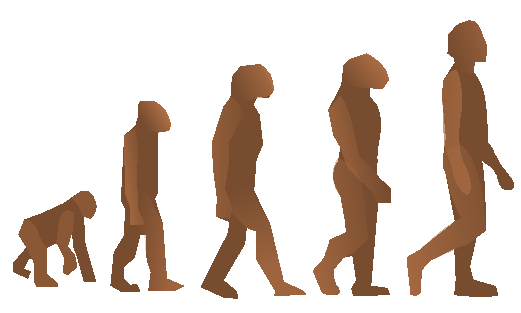
\includegraphics[width=2cm]{evolution_steps-vectorial}
   \caption{Vectorial image}\
 \end{wrapfigure}	
 
 \noindent\verb!\usepackage{wrapfig}!\\
 This then gives you access to:\\
 \verb!\begin{wrapfigure}[lineheight]{alignment}{width}!
 \\
 Alignment can normally be either 'l' for left, or 'r' for right. Lowercase 'l' or 'r' forces the figure to start precisely where specified (and may cause it to run over page breaks), while capital 'L' or 'R' allows the figure to float. If you defined your document as twosided, the alignment can also be 'i' for inside or 'o' for outside, as well as 'I' or 'O'. The width is obviously the width of the figure. The example above was introduced with: 
 \lstset{language=TeX, numbers=none, morekeywords={begin,includegraphics,caption}, caption=Wrapfig example, label=lst:latex_example}
 \begin{lstlisting}
 	\begin{wrapfigure}{l}{2.5cm}
 	  \centering
 	    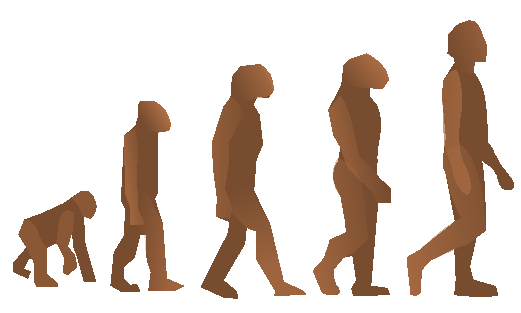
\includegraphics[width=2cm]{evolution_steps-vectorial}
 	  \caption{Vectorial image}
 	\end{wrapfigure}	
 \end{lstlisting}

% subsection inserting_images_wrapped_with_text (end)

% section floats_figures_and_captions (end)


\section{Text Formatting} % (fold)
\label{sec:text_formatting}

% section text_formatting (end)


\section{Generating PDFs from \texttt{LaTeX}} % (fold)
\label{sec:generating_pdfs_from_latex}

\subsection{Generating PDFs with pdflatex} % (fold)
\label{ssec:generating_pdfs_with_pdflatex}

You may create PDF files either by using \verb!latex! to generate a DVI file, and then use one of the many DVI-2-PDF converters, such as \verb!dvipdfm!.

Alternatively, you may use \verb!pdflatex!, which will immediately generate a PDF with no intermediate DVI or PS files. In some systems, such as Apple, PDF is already the default format for \texttt{LaTeX}. I strongly recommend you to use this approach, unless you have a very good argument to go for \verb!latex! + \verb!dvipdfm!.

A typical pass for a document with figures, cross-references and a bibliography would be:
\begin{verbatim}
$ pdflatex template
$ bibtex template
$ pdflatex template (twice)
\end{verbatim}
\begin{sloppypar}
You will notice that there is a new PDF file in the working directory called \verb!template.pdf!. Simple :)
\end{sloppypar}


Please note that, to be sure all table of contents, cross-references and bibliography citations are up-to-date, you must run \verb!latex! once, then \verb!bibtex!, and then \verb!latex! twice.
% section generating_pdfs_with_pdflatex (end)

\subsection{Dealing with Images} % (fold)
\label{sub:dealing_with_images}

You may process the same source files with both \verb!latex! or \verb!pdflatex!. But, if your text include images, you must be careful. \verb!latex! and \verb!pdflatex! accept images in different (exclusive) formats.  For \verb!latex! you may use EPS ou PS figures. For \verb!pdflatex! you may use JPG, PNG or PDF figures.  I strongly recommend you to use PDF figures in vectorial format (do not use bitmap images unless you have no other choice).
% subsection dealing_with_images (end)


\subsection{Creating Source Files Compatible with both latex and pdflatex} % (fold)
\label{ssec:creating_source_files_compatible_with_both_latex_and_pdflatex}

Do not include the extension of the file in the \verb!\includegraphics! command. E.g., use\\
\verb!\includegraphics{evolution_steps}!\\
and not\\
\verb!\includegraphics{evolution_steps.png}!.\\
If you use the first form, \verb!latex! or \verb!pdflatex! will add an appropriate file extension.

This means that, if you plan to use only \verb!pdflatex!, you need only to keep (preferably) a PDF version of all the images. If you plan to use also \verb!latex!, then you also need an EPS version of each image.\\
% subsection creating_source_files_compatible_with_both_latex_and_pdflatex (end)

% section generating_pdfs_from_latex (end)

{\Large To be included in the sections above} \\

If you are writing only one or two documents and aren't planning on writing more on the same subject for a long time, maybe you don't want to waste time creating a database of references you are never going to use. In this case you should consider using the basic and simple bibliography support that is embedded within \texttt{LaTeX}.

\texttt{LaTeX} provides an environment called \textbf{thebibliography} that you have to use where you want the bibliography; that usually means at the very end of your document, just before the \verb!\end{document}! command. Here is a practical example:

\begin{verbatim}
\begin{thebibliography}{9}

\bibitem{lamport94}
  Leslie Lamport,
  \emph{\LaTeX: A Document Preparation System}.
  Addison Wesley, Massachusetts,
  2nd Edition,
  1994.

\end{thebibliography}
\end{verbatim}

To actually cite a given document is \textit{very} easy. Go to the point where you want the citation to appear, and use the following: \verb!\cite{citekey}!, where the citekey is that of the bibitem you wish to cite, e.g \verb!~\cite{lamport94}!.  When \texttt{LaTeX} processes the document, the citation will be cross-referenced with the bibitems and replaced with the appropriate number citation. The advantage here, once again, is that LaTeX looks after the numbering for you.

When a sequence of multiple citations are needed, you should use a single \verb!\cite{}! command. The citations are then separated by commas. Note that you must not use spaces between the citations. Here's an result example \cite{strunk,chicago,texbook}.

Footnotes are a very useful way of providing extra information to the reader. Usually, it is non-essential information which can be placed at the bottom of the page. This keeps the main body of text concise.

The footnote facility is easy to use: \verb!\footnote{Simple footnote}!\footnote{Simple footnote}. 

The tabular environment can be used to typeset tables with optional horizontal and vertical lines. LaTeX determines the width of the columns automatically. The first line of the environment has the form: 
\verb!\begin{tabular}[pos]{table spec}!

\begin{itemize}
\item[table spec] tells LaTeX the alignment to be used in each column and the vertical lines to insert.
\item[pos] can be used to specify the vertical position of the table relative to the baseline of the surrounding text. 
\end{itemize}

The number of columns does not need to be specified as it is inferred by looking at the number of arguments provided. It is also possible to add vertical lines between the columns here. 

Some notes are important to followed, such as present in Table \ref{tab:results}: 
\begin{asparaenum}[i)]
	\item Not defined vertical lines;
	\item The legend must be on top;
	\item Use \verb!\toprule!, \verb!\midrule! and \verb!\bottomrule! to draw horizontal lines.
\end{asparaenum}
 
\begin{table}[ht]
	\caption{Table's rules.}
	\label{tab:results}
\centering
\begin{tabular}{llr}
\toprule
\multicolumn{2}{c}{Item} \\
\cmidrule(r){1-2}
Animal & Description & Price (\$) 
\\
\midrule
Gnat  & per gram & 13.65 \\
      & each     &  0.01 \\
Gnu   & stuffed  & 92.50 \\
Emu   & stuffed  & 33.33 \\
Armadillo & frozen & 8.99 \\
\bottomrule
\end{tabular}
\end{table}

\begin{sloppypar}
There are two ways to incorporate images into your \texttt{LaTeX} document, and both use the graphicx package by means of putting the command  \verb!\usepackage{graphicx}!  near the top of the \texttt{LaTeX} file, just after the documentclass command.
\end{sloppypar}

The two methods are

\begin{itemize}
\item  include only PostScript images (esp. 'Encapsulated PostScript') if your goal is a PostScript document using dvips;
\item include only PDF, PNG, JPEG and GIF images if your goal is a PDF document using pdflatex, \texttt{TeXShop}, or other PDF-oriented compiler. 
\end{itemize}

Some PNG images within my \texttt{LaTeX} document. The quality of the image files is sufficient and the result using \texttt{LaTeX} and viewing the resulting DVI file is quite looks good.

To get the best quality of the images in  PDF files I'd recommend using vector-based graphics for images. The best format to save images in is .pdf, see Figure \ref{fig:ra-vectorial}. With programs like \texttt{Inkscape}, you can draw as you would in MS Paint (and do much more), and because the images are vector-based instead of pixel-based, their quality should be preserved when converting to PDF in any way.    

In all cases, each image must be in an individual 1-image file; no animation files or multipage documents. 

There are two different ways to place two figures/tables side-by-side. The subfigure package provides functionality to arrange figures and tables next to each other, within the usual figure-floating-environment. Subfigure will alphabetically number your subfigures and you have access to the complete reference as usual through \verb!\ref{fig:subfig1}!, Figure \ref{fig:figura-completa}, or to the letter only through \verb!\subref{fig:subfig1}!, ~\subref{fig:ra-vectorial}, or either \verb!\ref{fig:ra-raster}!, Figure \ref{fig:ra-raster}.

\begin{figure}[htbp]
	\centering
    \subfigure[Vectorial] {
		\label{fig:ra-vectorial}
		
\includegraphics[width=0.4\textwidth]{ra-vectorial}
    }
\qquad\qquad
    \subfigure[Raster] {
		\label{fig:ra-raster}
		
\includegraphics[width=0.4\textwidth]{ra-raster}
    }
  \caption{Subfigure example with vectorial and no-vectorial images}
  \label{fig:figura-completa}
\end{figure}


Using the package listings you can add non-formatted text as you would do with \verb!\begin{verbatim}! but its main aim is to include the source code of any programming language within your document. If you wish to include pseudocode or algorithms see \href{http://en.wikibooks.org/wiki/LaTeX/Algorithms_and_Pseudocode}{LaTeX/Algorithms\_ and\_Pseudocode}, as Listing ~\ref{code:test}.

\begin{minipage}{\textwidth}
\lstset{language=R,numbers=left}
\begin{lstlisting}[
    frame=trBL,escapechar=|,
    caption={R-Code (Test).},
    label={code:test}
]
# comment
square <- function(x) {
    x^2
    % |$x^{2}$|
}

# nerv
x <- c(1:100)
y <- square(x)
\end{lstlisting}
\end{minipage}

\section{Equations}

Typesetting mathematics is one of \texttt{LaTeX}'s greatest strengths. It is also a large topic due to the existence of so much mathematical notation. It is recommend to read the following document available in \href{http://www.google.pt/url?sa=t&rct=j&q=&esrc=s&source=web&cd=1&cad=rja&ved=0CB4QFjAA&url=ftp%3A%2F%2Fftp.ams.org%2Fpub%2Ftex%2Fdoc%2Famsmath%2Fshort-math-guide.pdf&ei=DkScUOm8IJC5hAei7oGQDg&usg=AFQjCNEHl1pXuurNmXAdqfC0z-pPAbDyUw}{Short Math Guide for LaTeX - AMS - American Mathematical Society}.

\section{Page orientation}

\begin{sloppypar}
The default page layout is ``portrait'', but sometimes it is still useful/necessary to have the whole document or only single pages changed to ``landscape''. The latter might be due to a large table or figure. If you want to make appear the left side up, better readable on screen, the pdflscape-package will do it:
\verb!\usepackage{pdflscape}!
\end{sloppypar}
and again:
\begin{verbatim}
\begin{landscape}
...
\end{landscape}
\end{verbatim}

or, 
\verb!\includepdf[landscape=true,pages={1}]{example.pdf}!

to put the page in ``landscape'', while the rest will remain in ``portrait'' orientation. Nevertheless, the header/footer will also be changed in orientation.

\centering{\textbf{Written by Matilde Pós-de-Mina Pato with collaboration of Nuno Datia, \\2012 October}}